
%(BEGIN_QUESTION)
% Copyright 2011, Tony R. Kuphaldt, released under the Creative Commons Attribution License (v 1.0)
% This means you may do almost anything with this work of mine, so long as you give me proper credit

The following P\&ID shows a FOUNDATION Fieldbus {\it cascade} control system for regulating liquid level in a tank -- a level controller provides a ``remote setpoint'' signal to a flow controller, which then regulates how rapidly liquid flows out of the tank:

$$\includegraphics[width=15.5cm]{i00437x01.eps}$$

A function block diagram shows how the signals interconnect in this Fieldbus control system:

$$\includegraphics[width=15.5cm]{i00437x02.eps}$$

\filbreak

Based on the information presented, determine which of the following {\it timing diagrams} matches this Fieldbus segment:

$$\includegraphics[width=15.5cm]{i00437x04.eps}$$

$$\includegraphics[width=15.5cm]{i00437x03.eps}$$  % This is the correct diagram!

$$\includegraphics[width=15.5cm]{i00437x05.eps}$$ 

$$\includegraphics[width=15.5cm]{i00437x06.eps}$$ 

\underbar{file i00437}
%(END_QUESTION)





%(BEGIN_ANSWER)

$$\includegraphics[width=15.5cm]{i00437x03.eps}$$  % This is the correct diagram!

%(END_ANSWER)





%(BEGIN_NOTES)

A helpful problem-solving strategy is to use colors to designate which function blocks reside in the same field instrument:

$$\includegraphics[width=15.5cm]{i00437x07.eps}$$  

One clue to identifying the correct macrocycle schedule is identifying which function blocks must be compelled to broadcast their data over the Fieldbus network and which blocks don't need to broadcast data to the network at all.  This is a function of block location (i.e. which instrument it's located in).  Note, for example, how AI1 and PID1 are both located in the same device (LT-51), and therefore there is no need to broadcast AI1's output data to PID1.  Likewise, PID2 and AO are both located in the valve positioner FV-63, and so there is no need for PID2 to broadcast its output to AO, or for AO to broadcast its BKCAL\_OUT data to PID1.

\vskip 10pt

{\bf Blocks needing CD tokens to broadcast data to the Fieldbus network:}
\item{} PID1
\item{} AI2
\item{} PID2
\end{itemize}

\vskip 10pt

{\bf Blocks needing no CD token to broadcast data:}
\item{} AI1
\item{} AO
\end{itemize}

Based on these lists, the first and last macrocycles cannot be correct because they both show CD tokens issued to the AI1 and AO blocks.

\vskip 10pt

Examining the middle two timing diagrams, we now ask ourselves which one is the most reasonable in terms of ordering.  Of these, \#2 is more reasonable than \#3 because \#3 has PID1 broadcasting its output signal as a remote setpoint to PID2 {\it after} PID2 has already sent its command signal to the valve.  This would technically work, but it would require two full macrocycles for total information throughput, whereas the scheduling of \#2 would only require one macrocycle to get the same job done.


%INDEX% Fieldbus, function block: block execution sequence
%INDEX% Fieldbus, function block: macrocycle

%(END_NOTES)


